

\subsection{Verification through the Methods of Manufactured Solutions Results} 

%(insert table instead of equations, check comments in tex file for parameters)
%\begin{table}[h!]
%    \centering
%    \begin{tabular}{c|r}
%        $\bar{A}$ & test
%    \end{tabular}
%    \caption{Manufactured solution table for the first MMS test case}
%    \label{tab:MMS1_input}
%\end{table}
\begin{equation}
    M_x = 0.3 \left(
    \sum_{j=1}^5 R_{ij} +
    \sum_{j=1}^5 L_{ij} + 1
    \right) , B = 50
    \label{eqn:MMS_M_x}
\end{equation}

\begin{equation}
    \tilde{A} = \left(
    \sum_{j=1}^5 R_{ij} +
    \sum_{j=1}^5 L_{ij} + 1
    \right) , B = 0.3
    \label{eqn:MMS_A}
\end{equation}

\begin{align}
    \tilde{v}_{r,BCsImposed} = 
    \sum_{j=1}^3 R_{ij} +
    \sum_{j=1}^3 L_{ij} + 1, \\
    B = 2 , \\ 
    \tilde{v}_{r,BCsImposed}(\tilde{r}_{min}=\tilde{r}_{max}) = 0
    \label{eqn:MMS_vTh}
\end{align}

\begin{equation}
    \tilde{v}_{\theta} = \left(
    \sum_{j=1}^4 R_{ij} +
    \sum_{j=1}^4 L_{ij} + 1
    \right) , B = 50 
    \label{eqn:MMS_vTh}
\end{equation}

\begin{equation}
    \tilde{v}_{x} = 
    \sum_{j=1}^3 R_{ij} +
    \sum_{j=1}^3 L_{ij} + 1
    , B = 30 
    \label{eqn:MMS_vX}
\end{equation}

\begin{align}
    \tilde{p}_{diffBCsImposed} = 
    \sum_{j=1}^5 R_{ij} +
    \sum_{j=1}^5 L_{ij} + 1
    , B = 30 
    \label{eqn:MMS_p}
\end{align}

Figure \ref{fig:1} shows the manufactured solution for the mean flow profile. The tangent
summation method was used to generate the axial Mach number, the speed of sound, and the perturbation variables. The tangential Mach number was numerically
approximated by using the composite trapezoidal rule. The manufactured mean flow
profile is unique because it has been generated solely to verify SWIRL
and does not have physical significance. The “kinks” in the solution will allow a significant magnitude for the derivatives of these solutions.
\begin{figure}[h!]
    \centering
    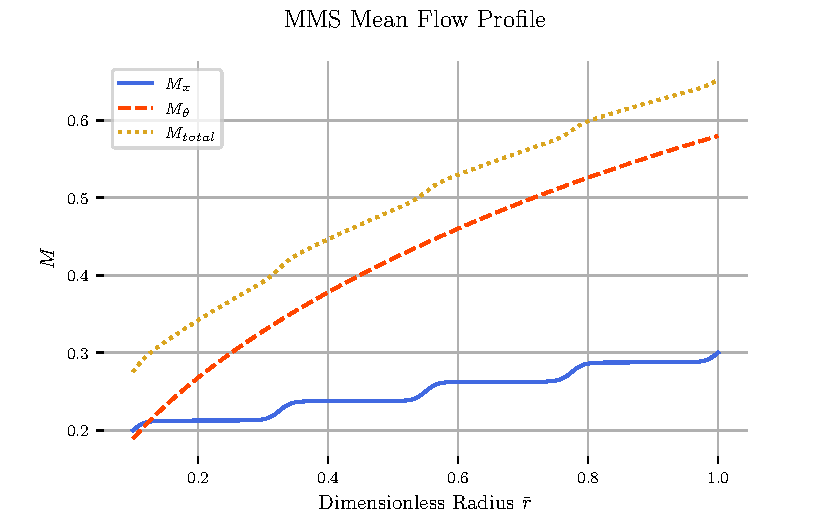
\includegraphics{../../../CodeRun/04-plotReport/tex-outputs/MMS1_mean_flow_profile.pdf}
    \caption{The manufactured mean flow test case using a summation of Tangents for $A$ and $M_x$}
    \label{fig:1}
\end{figure}

The results from the numerical integration are presented in Figure \ref{fig:5}. Although
the slope of the line appears linear, the TSM was still used to generate the MS for
the speed of sound. Denser grids were used to compute the error by iterating as 
grid spacing approaches zero. The difference between the expected speed of sound
to the actual speed of sound is shown in Figure \ref{fig:5a} as a function of 
radius. Note that the error reaches machine precision early in the 
iterations and approaches zero as more grid points are used.

\begin{figure}[h!]
    \centering
    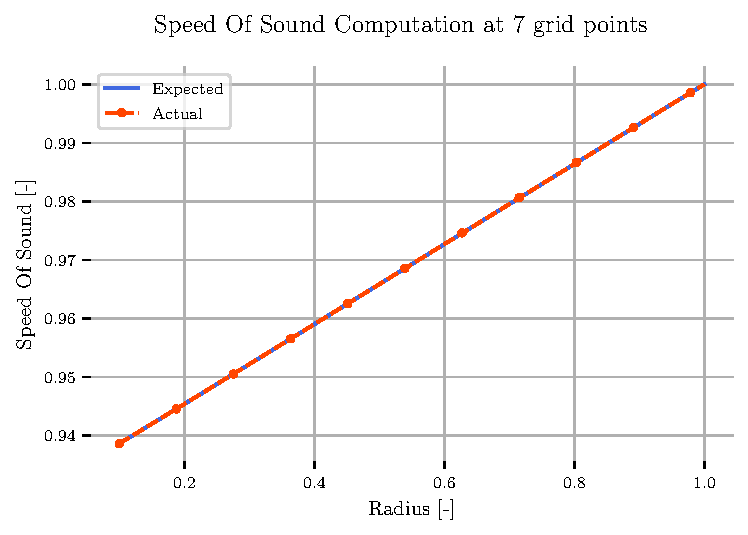
\includegraphics{../../../CodeRun/04-plotReport/tex-outputs/MMS1_SpeedOfSoundComparison1.pdf}
    \caption{ A comparison of the speed of sound, expected vs actual at the lowest grid to show similarities in solution}
    \label{fig:5}
\end{figure}


\begin{figure}[h!]
    \centering
    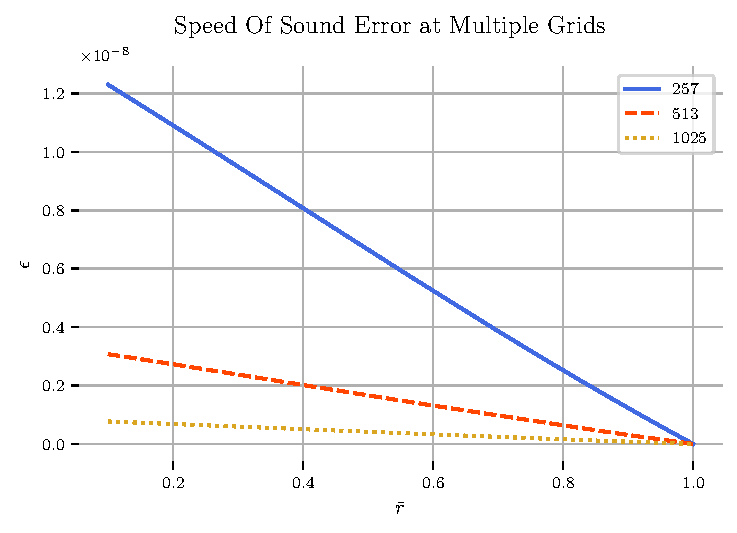
\includegraphics{../../../CodeRun/04-plotReport/tex-outputs/MMS1_SpeedOfSoundComparison2.pdf}
    \caption{ A comparison of the speed of sound error at three grid}
    \label{fig:5a}
\end{figure}

The error will decrease at a known rate depending on the type of numerical integration scheme. Since the composite trapezoidal rule has an order of accuracy
of 2, it is expected that the approximated order of accuracy will approach two as the
error approaches zero. This behavior is shown in Figure \ref{fig:8}, where the approximated
line is the L2 norm of the speed of sound error. The slope (i.e., the asymptotic rate of
convergence) approached two for numerical integration as the grid spacing decreases
(See Figure \ref{fig:9}) .

\begin{figure}[h!]
    \centering
    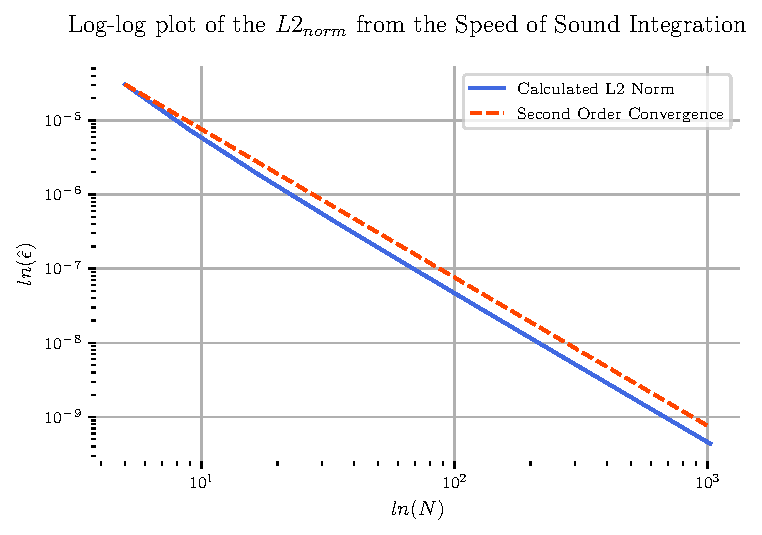
\includegraphics{../../../CodeRun/04-plotReport/tex-outputs/MMS1_SpeedOfSoundComparisonL2.pdf}
    \caption{L2 Norm comparison for the speed of sound integration for the compound trapezoidal rule}
    \label{fig:8}
\end{figure}

The manufactured solution used for the fluctuation variables in the MMS test case
is shown in Table \ref{tab:MMS1_input}. Recall that the variable B varies the slope around the
tangent function at each inflection point; the maximum amplitude of each tangent
function was A = 0.1 and was equally spaced between $\tilde{r}_{min}$-$\tilde{r}_{max}$.  
The boundary conditions for the perturbation variable $\tilde{v}_r$ were set 
using the fairing functions to impose boundary conditions. Fairing functions 
also set the derivative of the perturbation variable $\tilde{p}$. Only $\tilde{p}$
is affected by acoustic liners since it alters the rate of change of pressure at 
the walls, not the pressure or velocity. The subscripts $BCsImposed, diffBCsImposed$
state where the perturbation or its derivative value was altered to be uniform between the code and
the manufactured solution.


\begin{figure}[h!]
    \centering
    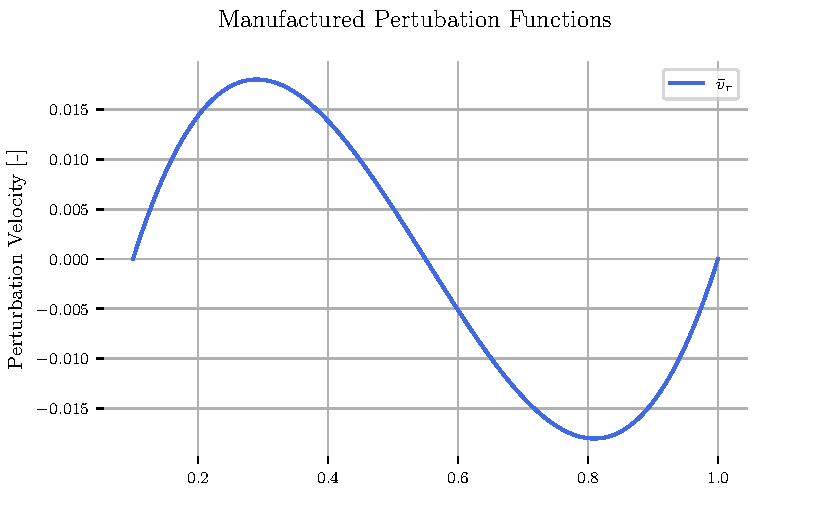
\includegraphics{../../../CodeRun/04-plotReport/tex-outputs/MMS1_perturbation_variables_vR.pdf}
\caption{The manufactured perturbation functions ,$v_r$}%, $v_x$, $v_{\theta}$, $p$}
    \label{fig:1a}
\end{figure}

\begin{figure}[h!]
    \centering
    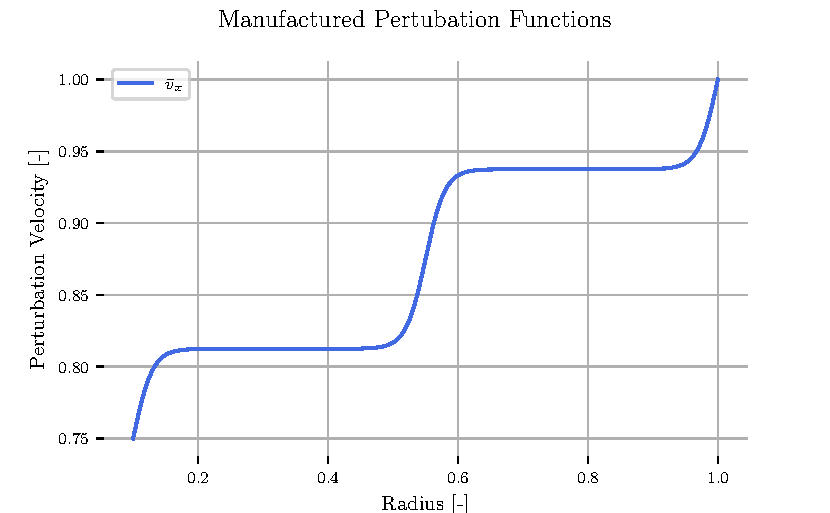
\includegraphics{../../../CodeRun/04-plotReport/tex-outputs/MMS1_perturbation_variables_vX.pdf}
\caption{The manufactured perturbation functions ,$v_x$}%, $v_x$, $v_{\theta}$, $p$}
    \label{fig:2a}
\end{figure}


\begin{figure}[h!]
    \centering
    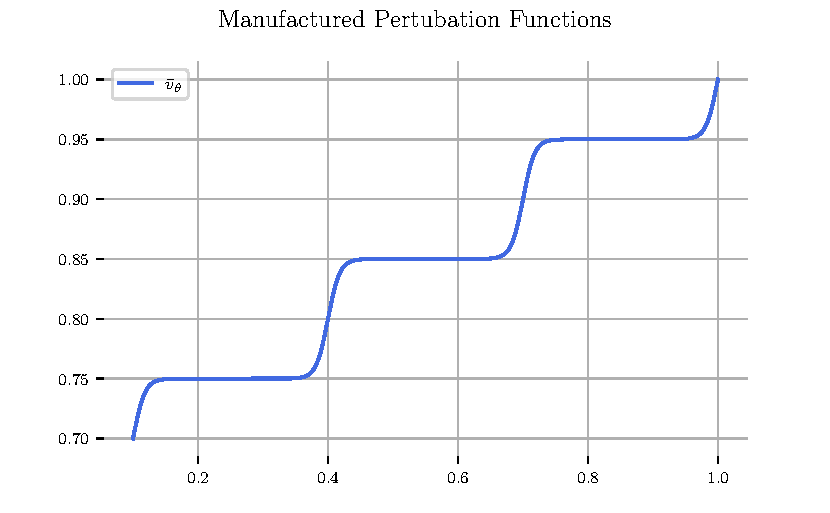
\includegraphics{../../../CodeRun/04-plotReport/tex-outputs/MMS1_perturbation_variables_vTh.pdf}
    \caption{The manufactured perturbation functions ,$v_{\theta}$}%, $v_x$, $v_{\theta}$, $p$}
    \label{fig:3a}
\end{figure}


\begin{figure}[h!]
    \centering
    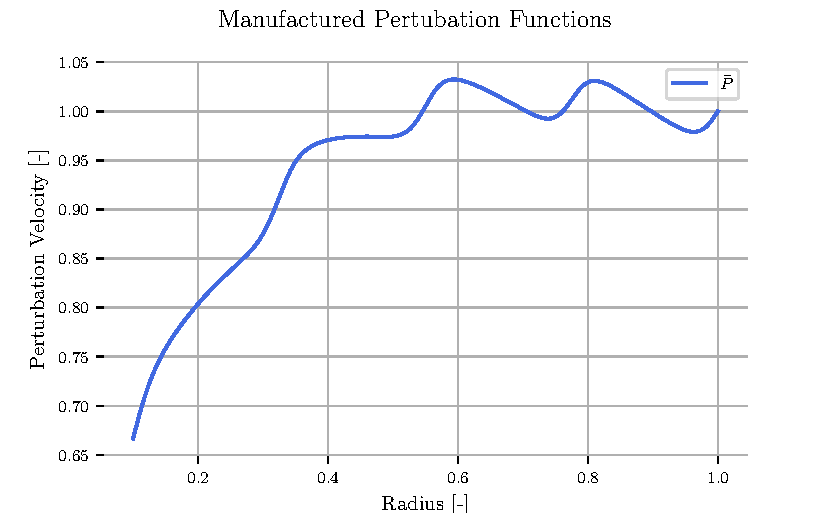
\includegraphics{../../../CodeRun/04-plotReport/tex-outputs/MMS1_perturbation_variables_Pr.pdf}
\caption{The manufactured perturbation functions ,$P$}%, $v_x$, $v_{\theta}$, $p$}
    \label{fig:4a}
\end{figure}



A second and fourth-order central differencing scheme for the LEE is used for 
the approximated radial derivatives and compared to the source terms generated 
for the MMS in Figure 5-10.The L2 norm and the asymptotic rate of convergence 
is shown for the two diffferencing schemes in 5-15 . 

The grid points were doubled, starting at 7 grid points and ending after 9 iterations with 1025 grid points. Both schemes do not have the order of accuracy down to machine precision but get down to $10^-6$
For the LEE, a second and fourth order central differencing scheme is used
for the approximated radial derivatives and then compared to the source terms 
generated for the MMS in Figure \ref{fig:6}. 
\begin{figure}[h!]
    \centering
    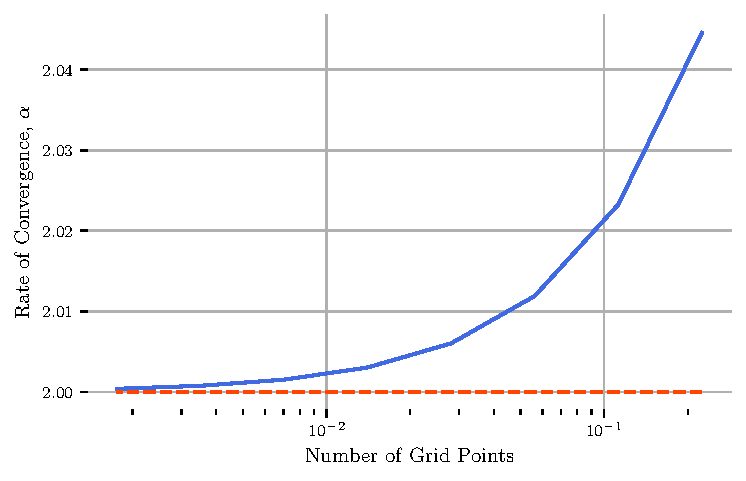
\includegraphics{../../../CodeRun/04-plotReport/tex-outputs/MMS1_SpeedOfSoundComparisonROC.pdf}
    \caption{ Speed of Sound Rate Of Convergence}
    \label{fig:SpeedOfSoundROC}
\end{figure}

\begin{figure}[h!]
    \centering
    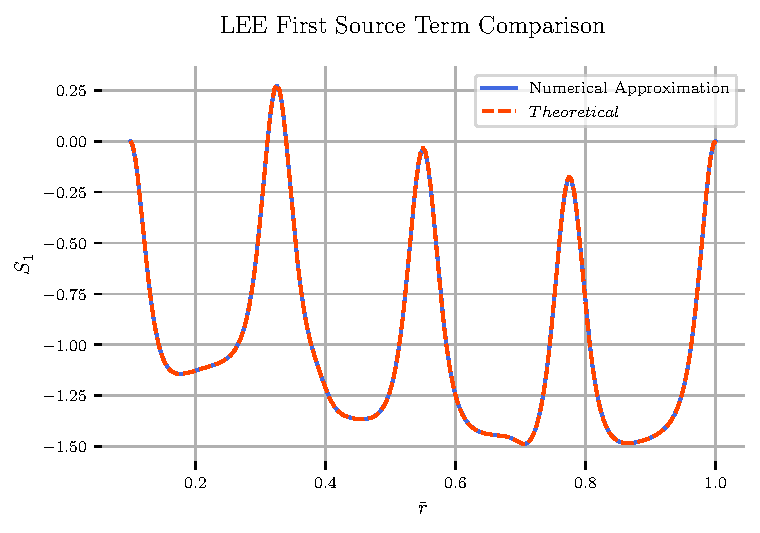
\includegraphics{../../../CodeRun/04-plotReport/tex-outputs/MMS1_SourceTermComparison1.pdf}
    \caption{Comparison of manufactured source term for the first linearized Euler equation}
    \label{fig:6}
\end{figure}

\begin{figure}[h!]
    \centering
    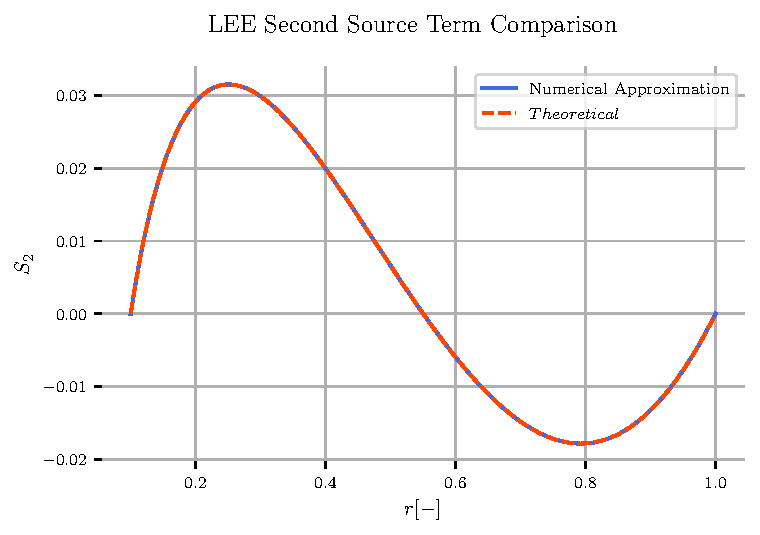
\includegraphics{../../../CodeRun/04-plotReport/tex-outputs/MMS1_SourceTermComparison2.pdf}
    \caption{Comparison of manufactured source term for the second linearized Euler equation}
\end{figure}

\begin{figure}[h!]
    \centering
    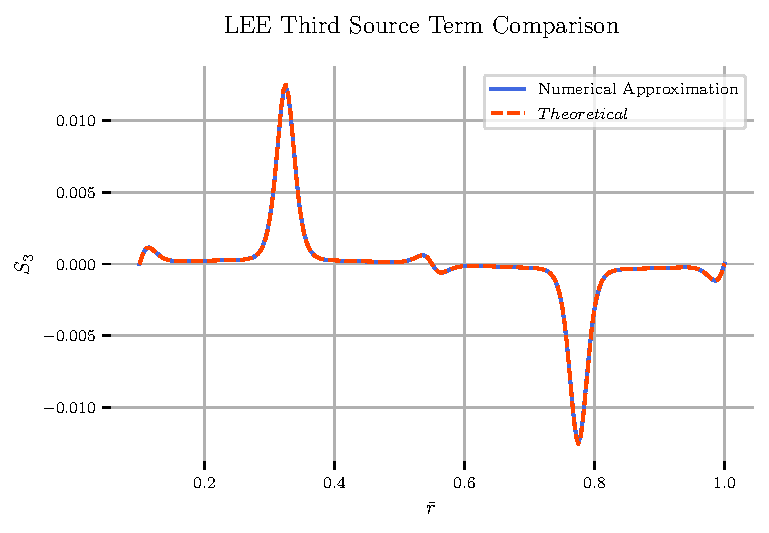
\includegraphics{../../../CodeRun/04-plotReport/tex-outputs/MMS1_SourceTermComparison3.pdf}
    \caption{Comparison of manufactured source term for the third linearized Euler equation}
\end{figure}

\begin{figure}[h!]
    \centering
    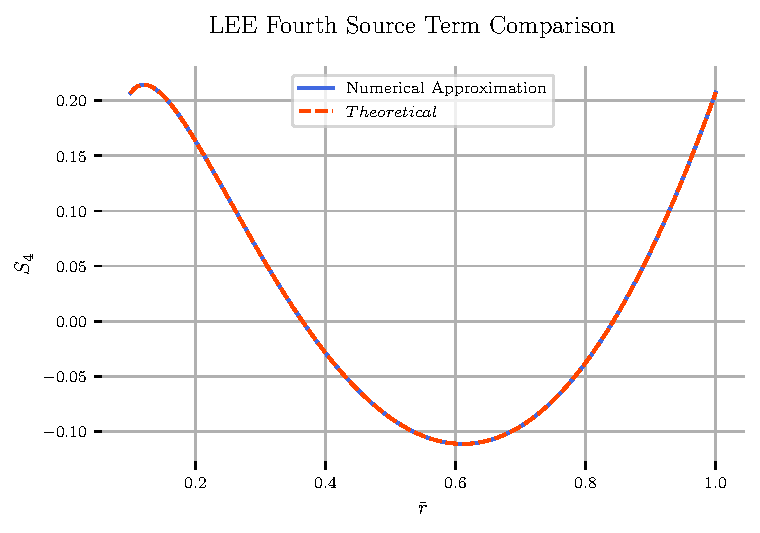
\includegraphics{../../../CodeRun/04-plotReport/tex-outputs/MMS1_SourceTermComparison4.pdf}
    \caption{Comparison of manufactured source term for the fourth linearized Euler equation}
\end{figure}




\begin{figure}[h!]
    \centering
    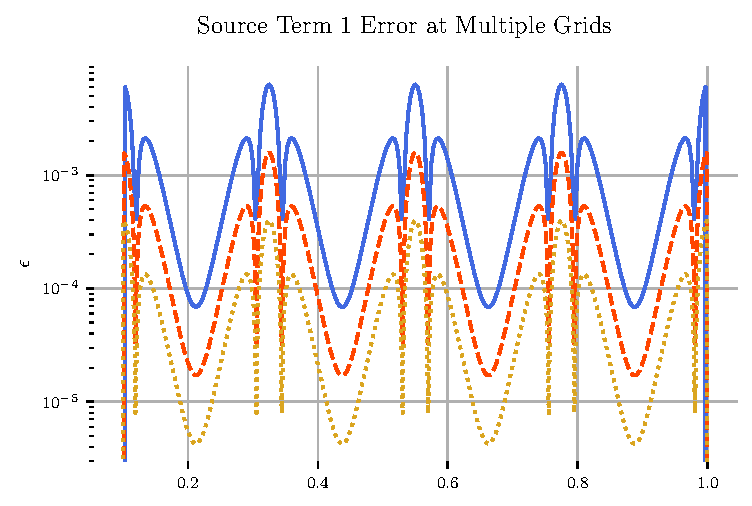
\includegraphics{../../../CodeRun/04-plotReport/tex-outputs/MMS1_SourceTermError1.pdf}
    \caption{LEE Source Term Error}
    \label{fig:7}
\end{figure}


\begin{figure}[h!]
    \centering
    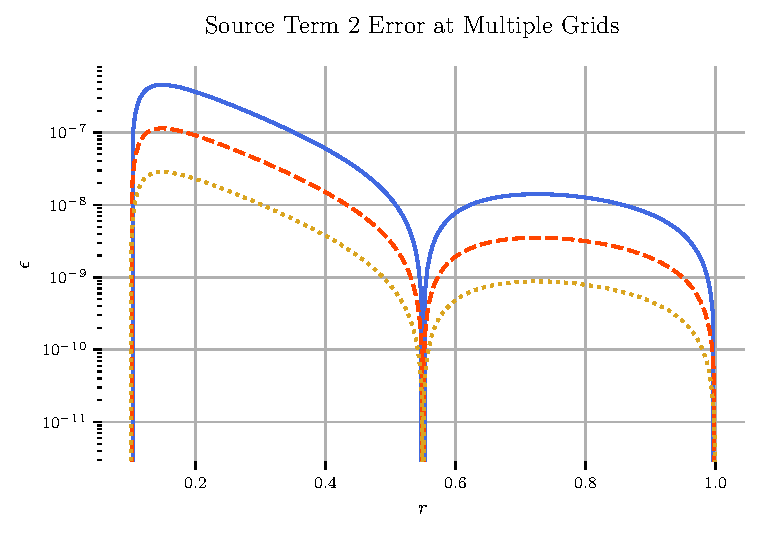
\includegraphics{../../../CodeRun/04-plotReport/tex-outputs/MMS1_SourceTermError2.pdf}
    \caption{LEE Source Term Error}
    \label{fig:7}
\end{figure}


\begin{figure}[h!]
    \centering
    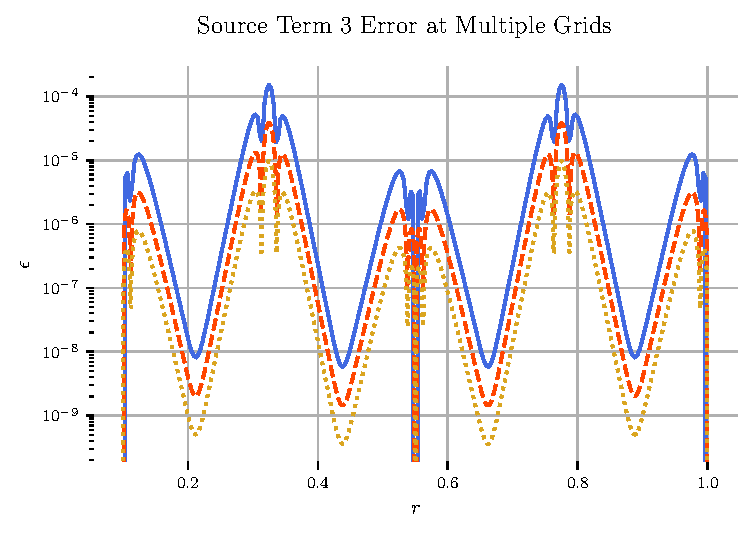
\includegraphics{../../../CodeRun/04-plotReport/tex-outputs/MMS1_SourceTermError3.pdf}
    \caption{LEE Source Term Error}
    \label{fig:7}
\end{figure}


\begin{figure}[h!]
    \centering
    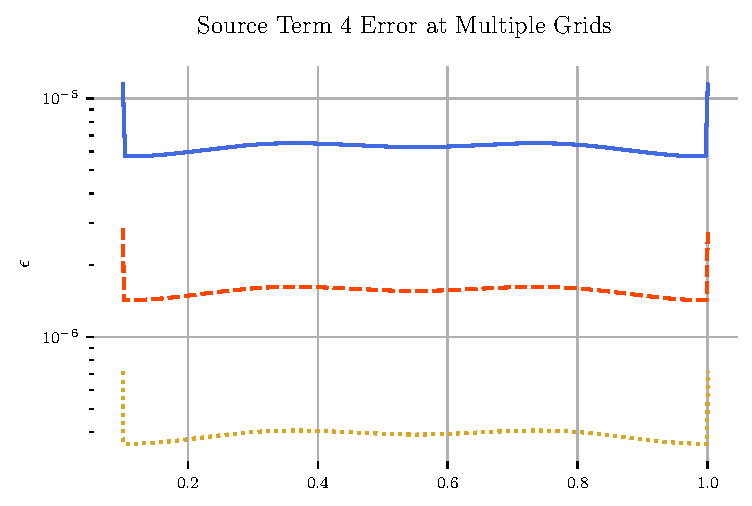
\includegraphics{../../../CodeRun/04-plotReport/tex-outputs/MMS1_SourceTermError4.pdf}
    \caption{LEE Source Term Error}
    \label{fig:7}
\end{figure}


\begin{figure}[h!]
    \centering
    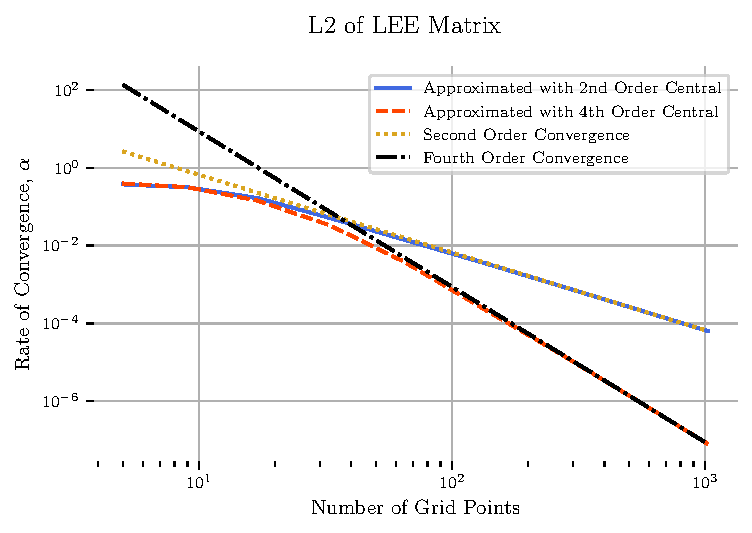
\includegraphics{../../../CodeRun/04-plotReport/tex-outputs/MMS1_LEE_L2.pdf}
    \label{fig:9}
\end{figure}

\begin{figure}[h!]
    \centering
    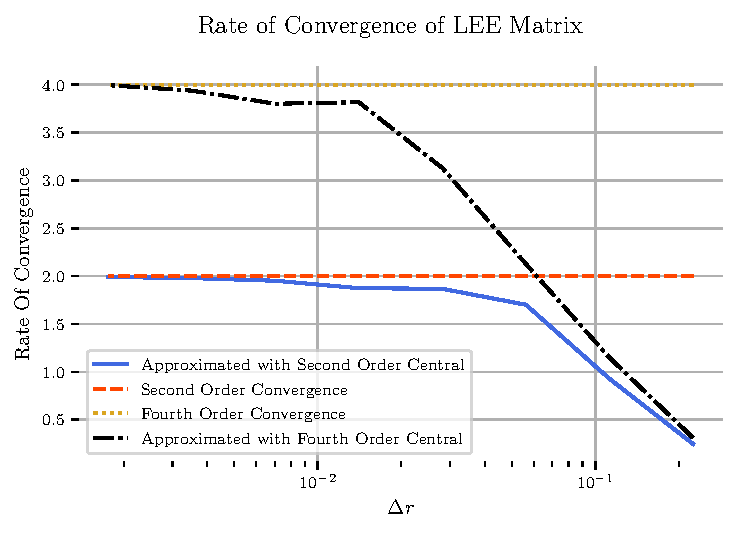
\includegraphics{../../../CodeRun/04-plotReport/tex-outputs/MMS1_LEE_ROC.pdf}
    \label{fig:9}

